\subsection{Logarithmic Signature}
\label{subsec:motion-capture-log-signature}

Another way to determine the shape space distance between two motions is to use the logarithmic signature method to find \(d_{\text{sig}_*}\) between all the curves, as defined in Equation \eqref{eq:signature-distance-metric}. We compute the logarithmic signature of each motion, normalize the signatures, and calculate the \(L^2\) norm of the difference between the normalized signatures. This distance is stored in a distance matrix, where the diagonal is zero since the distance between a motion and itself is zero.

\begin{figure}
    \centering
    \begin{subfigure}{\textwidth}
        \centering
        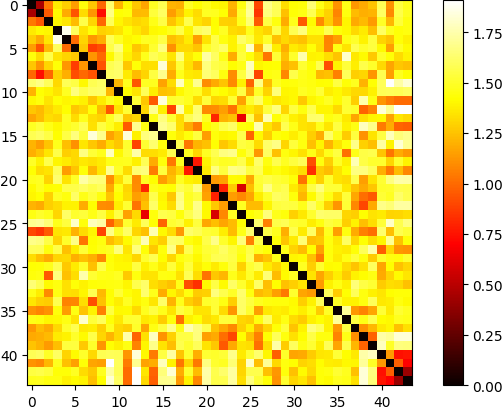
\includegraphics[width=0.53\textwidth]{figures/motion-capture-data/heatmaps/logsig_1.png}
        \caption{}
        \label{fig:heatmaps-logsig-1}
    \end{subfigure}
    \begin{subfigure}{\textwidth}
        \centering
        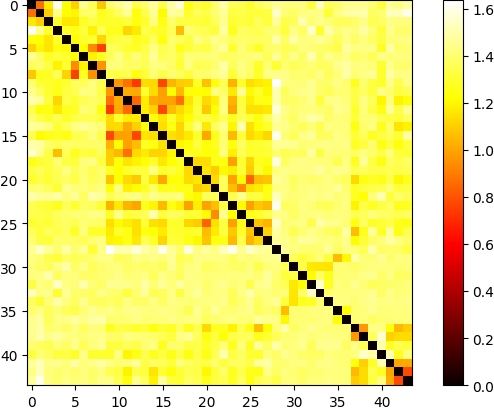
\includegraphics[width=0.53\textwidth]{figures/motion-capture-data/heatmaps/logsig_2.png}
        \caption{}
        \label{fig:heatmaps-logsig-2}
    \end{subfigure}
    \begin{subfigure}{\textwidth}
        \centering
        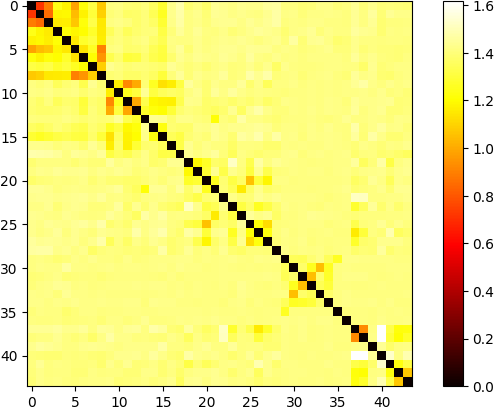
\includegraphics[width=0.53\textwidth]{figures/motion-capture-data/heatmaps/logsig_3.png}
        \caption{}
        \label{fig:heatmaps-logsig-3}
    \end{subfigure}
    \caption[Heatmap: Motion Capture Data Classification utilizing Logarithmic Signature]{Heatmaps of the distance matrix from motion capture data, where the distance matrix was created by the Logarithmic Signature and the \(L^2\) norm of these normalized signatures with truncation levels of: (a) 1, (b) 2, and (c) 3.}
    \label{fig:heatmaps-logsig}
\end{figure}

The results for three different truncation levels (1, 2, and 3) are shown in Figure \ref{fig:heatmaps-logsig}. In \ref{fig:heatmaps-logsig-1} there is significant noise, resembling Gaussian noise, indicating that it does not effectively distinguish between the motions. In \ref{fig:heatmaps-logsig-2} we see a block around "forward jump" and another block encompassing both "run/jog" and "walk" with a separate block forming at "climbing stairs". There is a significant distance between these and other motions. In \ref{fig:heatmaps-logsig-3} "forward jump" remains distinct, "run/jog" becomes distinct from "walk" and there are hints of "boxing" and "climbing stairs" being distinct.

These results show that higher truncation levels yield more detailed distinctions, enabling the method to better differentiate between various motions due to the increased nuanced information. Additionally, the logarithmic signature method highlights different aspects of the data compared to the reparameterization method, which is expected given the fundamental differences between the two approaches.